\noindent With reference to previous studies\cite{Fahrus1931THETUBES, Pries1992BloodHematocrit, SECOMB2013470} conducted, a consistent finding was observed that $\mu_{app}$ decreases substantially with decreasing tube diameters below around 300 $\mu$m and this well-known phenomenon is called the F{\aa}hr{\ae}us-Lindqvist effect. To observe whether the F{\aa}hr{\ae}us-Lindqvist effect exists in the micro-vascular networks from simulation data, graphs of relative apparent viscosity ($\mu_{rel}$) against haematocrit (H$_{D}$) and branch diameter (D$_{H}$) were plotted. From Figure \ref{Fahraeus-LindqvistEffectH}, if all the zero-haematocrit data points were excluded, there were 3 observations identified:

\begin{enumerate}
    \item Taking a horizontal viewpoint of the graph and disregarding the classification of PB, CB-L and CB-S, the overall $\mu_{rel}$ increases against $H_{D}$ except for one single outlier. 
    \item Based on a vertical viewpoint of the graph, a wide range of $\mu_{rel}$ is observed for a given $H_{D}$. This is related to the F{\aa}hr{\ae}us-Lindqvist effect which describes the non-monotonic variation of the relative apparent viscosity against vessel diameter at a fixed H$_{D}$.
    \item The data points of CB-L and CB-S are more or less overlapped while majority of the PB data points are at the bottom of the graph which indicates having relatively smaller $\mu_{rel}$. 
\end{enumerate}

\begin{figure}[H]
\centering
\begin{subfigure}{0.50 \textwidth}
    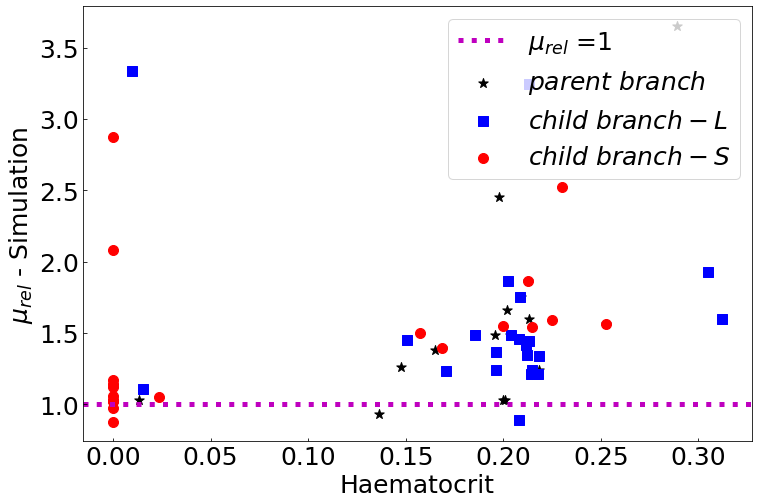
\includegraphics[width=1\textwidth]{images/Fahraeus-LindqvistEffectH.png}
    \caption{\textit{Graph of $\mu_{rel}$ against H$_{D}$ with classification of PB, CB-L and CB-S.} \label{Fahraeus-LindqvistEffectH}}
\end{subfigure}
\hfill
\begin{subfigure}{0.48 \textwidth}
    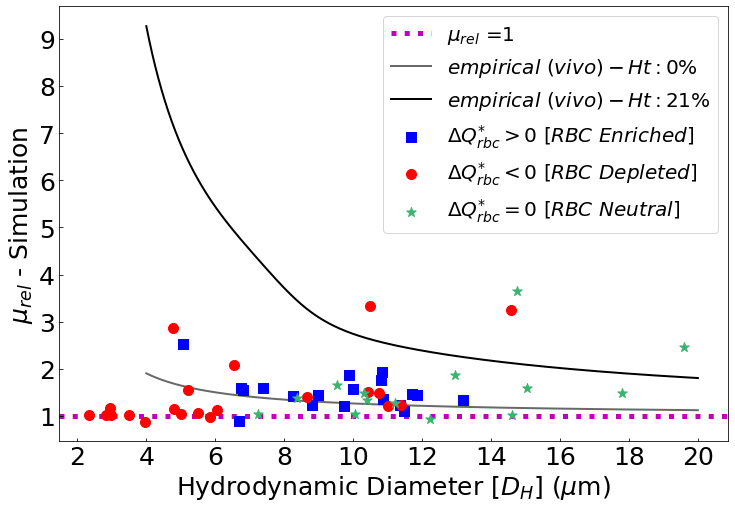
\includegraphics[width=1\textwidth]{images/Fahraeus-LindqvistEffectD.png}
    \caption{\textit{Graph of $\mu_{rel}$ against D$_{H}$ with classification of neutral, RBC-enriched and RBC-depleted branches} \label{Fahraeus-LindqvistEffectD}}
\end{subfigure}
\caption{\textit{Demonstration of the presence of F{\aa}hr{\ae}us-Lindqvist effect within micro-vascular networks from simulation data. The purple dotted line represents the ratio of apparent blood viscosity against plasma viscosity is equivalent to 1.} \label{Fahraeus-LindqvistEffects}}
\end{figure}

\noindent For Figure \ref{Fahraeus-LindqvistEffectD}, two empirical lines with a fixed H$_{D}$ of 0\% and 21\% were included to observe how much the simulation data deviates from empirical prediction. These two values were selected because the majority of the RBC-depleted and RBC-enriched branches were found around either the 0\% or 21\% haematocrit levels as shown in Figure \ref{DisproportionalityIndexHD}. However, we do have to take note that this may not be an accurate evaluation as some branches do not have an exact haematocrit of either 0\% or 21\%. In Figure \ref{Fahraeus-LindqvistEffectD}, it was observed that the majority of the simulation data do significantly deviate from empirical predictions and a vast majority of the RBC-depleted branches have a lower apparent blood viscosity than the RBC-enriched branches. Furthermore, branch diameters smaller than 8$\mu$m (diameter of a freely suspended human RBC) tend to have a greater deviation between simulation data and empirical predictions compared to branch diameters larger than 8$\mu$m. \\

\noindent According to these observations mentioned above, it implies that the simulation data was unable to clearly demonstrate the presence of F{\aa}hr{\ae}us-Lindqvist effect. The primary reason could be the difference in branch length ($L$) within the micro-vascular networks from simulation data compared to previous experimental studies. 